\documentclass{article}

\usepackage{amsmath} % math stuff
\usepackage{amssymb} % math stuff
\usepackage{array} % equations and stuff
\usepackage{bm} % bold math
%\usepackage{booktabs} % extra table rule options
%\usepackage{caption} % suppressed table numbering; incompatible with revtex, and longtable, I think
\usepackage{comment} % comment environment
%\usepackage{enumitem} % customization of enumeration, itemize, and description
\usepackage[T1]{fontenc} % font encoding for special characters, must also use scalable font package
\usepackage[margin=0.8in]{geometry} % paper sizes and margins (but be careful not to mess up pre-defined pages)
\usepackage{graphicx} % for graphics
%\usepackage{helvet} % default font is the helvetica postscript font
\usepackage{layouts} % print units like widths
\usepackage{lipsum} % lorem ipsum filler text
\usepackage{lmodern} % scalable font?
\usepackage{longtable} % multi-page tables
\usepackage{makecell} % specify line-breaks in table cells
\usepackage{mathrsfs} % math script font
\usepackage{mhchem} % easier chemical formula
\usepackage{microtype} % allows disabling of ligatures
%\usepackage{newcent} % new century schoolbook font
\usepackage{nicefrac}
\usepackage{numprint} % print and format (large) numbers
\usepackage{parskip} % removes paragraph indentation, and adjusts paragraph skip, as well as list items
\usepackage{pdfpages} % add pdf files as pages
%\usepackage{setspace} % adjust text spacing and indents
\usepackage{siunitx} % decimal alignment
\usepackage{subfigure} % divided figures
%\usepackage{tabu} % extra table options
\usepackage{textcomp} % symbols
\usepackage{threeparttablex} % better footnotes with longtable
\usepackage{titling} % title placement
\usepackage{ulem} % strikethrough text
%\usepackage{url} % superceded by hyperref
\usepackage{verbatim} % verbatim environment
\usepackage{xcolor} % colors and color boxes
\usepackage{xspace} % commands that don't eat up white space
\usepackage{hyperref} % links and page setup; should always come last

\hypersetup{
 bookmarks=true,
 colorlinks=true,
 citecolor=blue,
 linkcolor=blue,
 urlcolor=blue,
 pdfstartview={XYZ null null 1.0} % default open view is 100%
}

\DisableLigatures[f,t]{encoding = T1} % disable ff, fi, fl, tt ligatures; without options, it also disables -- = endash
\renewcommand{\arraystretch}{1.0} % extra vertical (and horizontal?) space in tables

% define centered, left- and right-aligned columns with specified widths
\newcommand{\PreserveBackslash}[1]{\let\temp=\\#1\let\\=\temp}
\newcolumntype{C}[1]{>{\PreserveBackslash\centering}p{#1}}
\newcolumntype{L}[1]{>{\PreserveBackslash\raggedright}p{#1}}
\newcolumntype{R}[1]{>{\PreserveBackslash\raggedleft}p{#1}}

\begin{document}

\pagestyle{empty} % don't number pages

% custom title
\begin{center}
{\LARGE Classic Riddler}

\vspace{0.15in}

{\Large 23 April 2021}
\end{center}


\section*{Riddle:}

Riddler Nation's neighbor to the west, Enigmerica, is holding an election between two candidates, A and B.
Assume every person in Enigmerica votes randomly and independently, and that the number of voters is very, very large.
Moreover, due to health precautions, 20 percent of the population decides to vote early by mail.

On election night, the results of the 80 percent who voted on Election Day are reported out.
Over the next several days, the remaining 20 percent of the votes are then tallied.

What is the probability that the candidate who had fewer votes tallied on election night ultimately wins the race?


\section*{Solution:}

For some number $N$ of choices being made between 2 options with a determined probability $p$, the distribution of outcomes is a binomial distribution.
For a sufficiently large number ($N\gtrsim25$ I think) as well as a sufficiently large product $Np$, then the distribution can be approximated by the (continuous) normal distribution.
In this problem, because it is specified that the number of voters ($N$) is very large, and the probability of each voter to choose a given candidate ($p$) is 0.5, both of these conditions hold.
Modeling the vote distribution as a normal distribution makes computation much simpler (relatively).

The important thing to note about the normal distribution is that the standard deviation $\sigma$ (the width) of the distribution scales as $\sqrt{N}$.
In this case there are actually 2 distributions: the in-person voters (of whom there are $0.8N$) and the mail-in voters ($0.2N$).
The absolute widths are not known, but the relative width is important, which in this case is $\nicefrac{\sigma_{\rm{ip}}}{\sigma_{\rm{mi}}}=\sqrt{\nicefrac{0.8}{0.2}}=2$.

Given the relative standard deviations, the equations for the in-person ($P_{\rm{ip}}(x)$) and mail-in ($P_{\rm{mi}}(x)$) vote distributions can be given as follows (given some general mean $\mu$):

\[
P_{\rm{ip}}(x)=\frac{1}{2\sqrt{2\pi}}e^{-\frac{(x-\mu)^{2}}{8}}
\]
\[
P_{\rm{mi}}(x)=\frac{1}{\sqrt{2\pi}}e^{-\frac{(x-\mu)^{2}}{2}}
\]

The probability that the total vote is different than the in-person vote is equivalent to the probability that a point on the second distribution is both farther from the mean and opposite side of the mean as a point on the first distribution.
This is done by transforming the variables, and integrating the points directly.
Here, the mean of the first distribution is taken to be 0.
Now the variable essentially becomes the vote differential in favor of a particular candidate.
The mean of the second distribution then becomes the first variable (which I will also change to $y$ instead of $x$).
The integration then arises from the area of the second distribution below 0 for values of $y$ above 0, and the area above 0 for values of $y$ below 0.
This is illustrated in the graph below.
Here, first distribution (mail-in) is shown in black and is twice as wide as the second distribution in blue.
The integrated area is shown in gray, and the second distribution is moved across and scaled according to the first distribution.

\vspace{0.1in}
\begin{center}
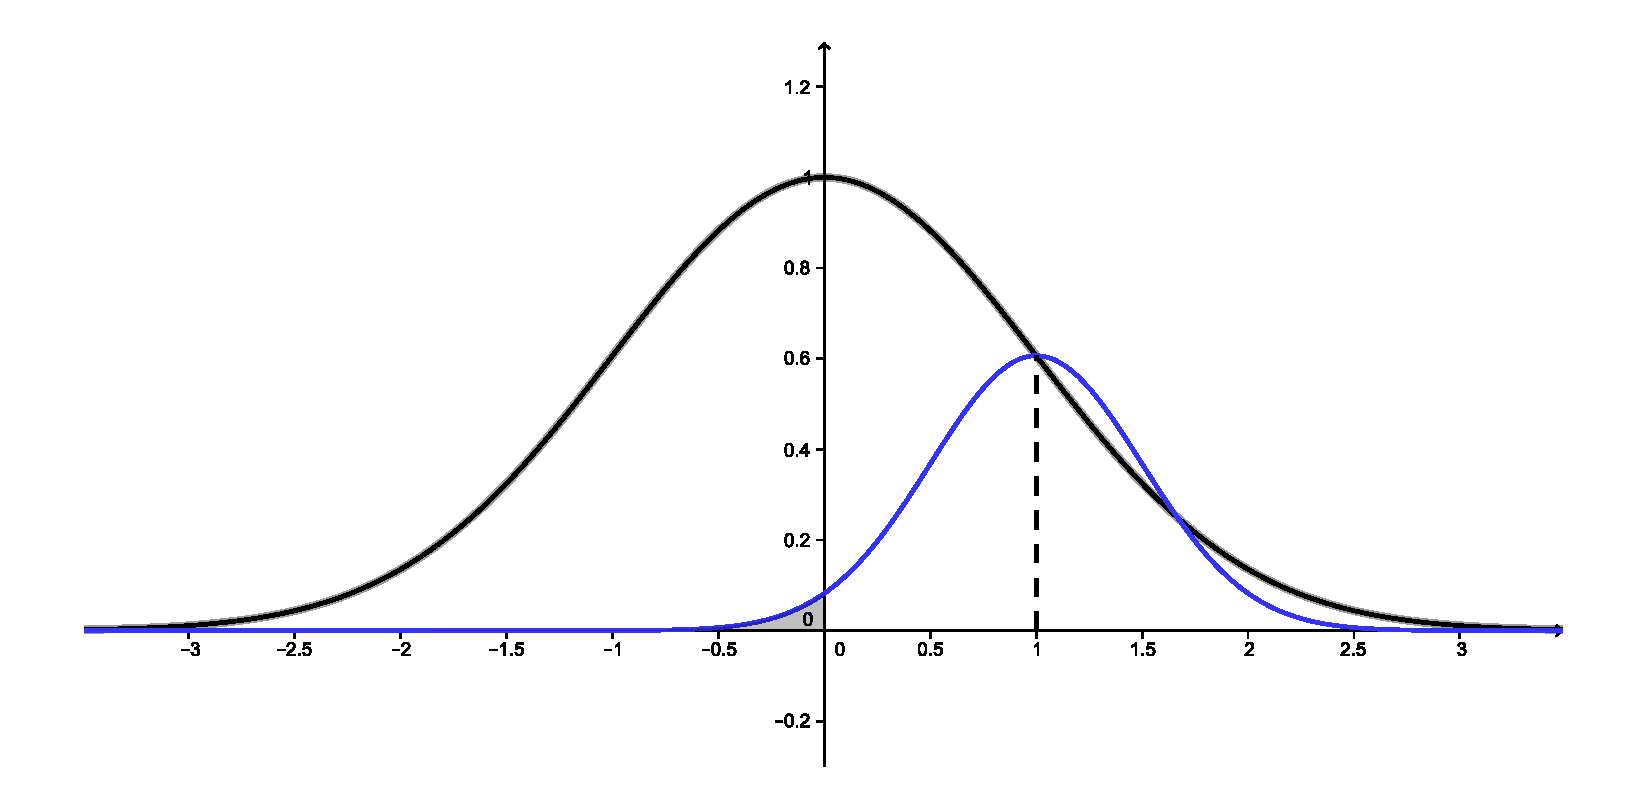
\includegraphics[width=6in]{graph.pdf}
\end{center}
\vspace{0.1in}

The actual integral that gives the solution is:

\[
2\cdot\int_{0}^{\infty}\int_{-\infty}^{0}\frac{1}{\sqrt{2\pi}}e^{-\frac{(x-y)^{2}}{2}}\frac{1}{2\sqrt{2\pi}}e^{-\frac{y^{2}}{8}}\,dx\,dy
\]

I am reliably informed by Wolfram Alpha that the solution to this integral is

\[
\frac{\tan^{-1}(\nicefrac{1}{2})}{\pi}
\]

This leads me to believe (though I cannot nearly prove) that the general solution for a fraction $f$ of in-person voters is

\[
\frac{\tan^{-1}\sqrt{\nicefrac{(1-f)}{f}}}{\pi}
\]

So the solution is
\fcolorbox{red}{white}{$\bm{{\nicefrac{\tan^{-1}(1/2)}{\pi}\approx0.1476}}$}\,.




\end{document}